\appendix
\clearpage
\addappheadtotoc
\appendixpage
\chapter{Herramienta IPerf}
IPerf es una herramienta de evaluación del rendimiento en las comunicaciones en una red. Esta evaluación la llevará a cabo por medio de del trafico generado y el tiempo transcurrido entre cliente servidor. Hay distintas posibilidades a la hora de generar tráfico, tráfico TCP por defecto o UDP indicándolo debidamente en sus parámetros opcionales. La arquitectura de la aplicación se estructura en un nodo cliente y otro servidor. En función de la parte de la herramienta tendrá una serie de parámetros y opciones con respecto a la otra parte en cuestión.\newline
\newline
\begin{figure}[!htb]
  \centering
    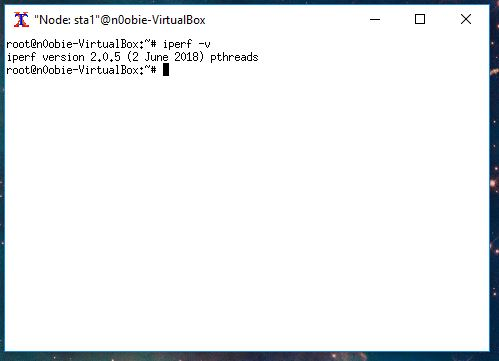
\includegraphics[width=0.7\linewidth]{./img/anexos/1.JPG}
    \caption{Versión de IPerf a utilizar.}
  \label{fig:yo}
\end{figure}
\section{Opciones}
Parámetros parte \textbf{servidor}, para especificar que se trata de esta parte de la herramienta hay que indicarlo con la opción \textbf{-s} ó \textbf{--server}. Se van a indicar los más importantes, si se requiere más información consulte la pagina del desarrollador.
\begin{center}
    \url{https://iperf.fr/iperf-doc.php}
\end{center}
\newpage
Opciones en el servidor:
\begin{itemize}
    \item -D, como servicio (En Unix como un daemon).
    \item -R, remover el servicio.
    \item -u, recibir datagramas UDP en vez de TCP por defecto.
    \item -P, indicando el número de conexiones simultáneas.
    \item -m, muestra MTU.
    \item -w, especifica el tamaño de Ventana (TCP window size).
    \item -f,   [bkmBKB] Cambiar unidades los resultados en \textbf{b}its/s, \textbf{k}ilobits/s, \textbf{m}egabytes/s, \textbf{B}ytes/s, \textbf{K}iloBytes/s, \textbf{M}egaBytes/s.
\end{itemize}
Parámetros parte \textbf{cliente}, para especificar que se trata de esta parte de la herramienta hay que indicarlo con la opción \textbf{-c} ó \textbf{--client}. Se van a indicar los más importantes, si se requiere más información, como se ha indicado anteriormente, consulte la pagina del desarrollador.\newline
\newline
Opciones en el cliente:
\begin{itemize}
    \item -t, segundos tiempo duración transmisión. Hace más fiable la medida.
    \item -i, segundos especifica un intervalo, medido en segundos, en el cual se volverá a realizar la medición.
    \item -T, ttl especifica valor TTL.
    \item -m, muestra MTU.
    \item -w, especifica el tamaño de Ventana (TCP window size).
    \item -f,   [bkmBKB] Cambiar unidades los resultados en \textbf{b}its/s, \textbf{k}ilobits/s, \textbf{m}egabytes/s, \textbf{B}ytes/s, \textbf{K}iloBytes/s, \textbf{M}egaBytes/s.
\end{itemize}
\section{Ejemplo de uso}
Lo primero que debemos hacer es escoger dos nodos de la red y decidir quien va a ser el servidor y quien será el cliente. Una vez tomada esa decisión debemos poner a escuchar a la parte servidor. Esto lo haremos según hemos indicado antes. Podemos ver como el servidor está a la escucha en el puerto 5001.
\begin{figure}[!htb]
  \centering
    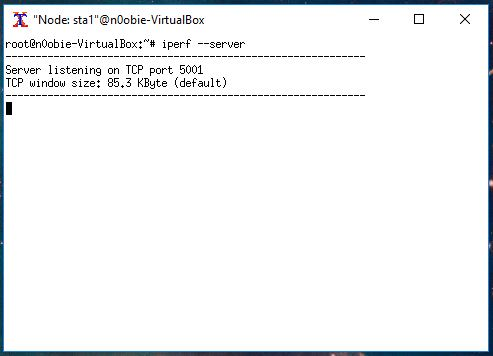
\includegraphics[width=0.5\linewidth]{./img/anexos/2.JPG}
    \caption{Levantar parte servidor.}
  \label{fig:yo}
\end{figure}
\newpage
Acto seguido vamos al otro nodo e indicamos su condición de cliente, a quien debe conectarse, y en el caso que lo queramos las configuraciones extras que consideremos oportunas.\newline
\newline
\begin{figure}[!htb]
  \centering
    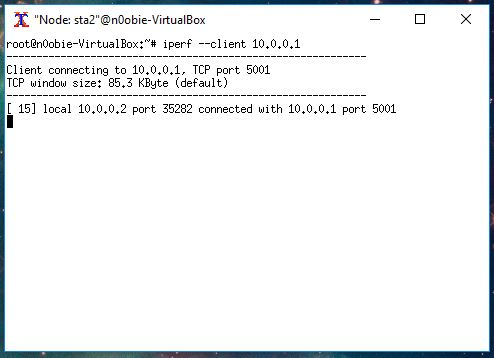
\includegraphics[width=0.7\linewidth]{./img/anexos/3.JPG}
    \caption{Levantar parte cliente y conectarla con el servidor.}
  \label{fig:yo}
\end{figure}
\newline
Una vez completado el test de performance podremos ver los resultados de ancho de banda obtenidos. En este caso nos lo indica en las unidades por defecto pero haciendo uso del flag -f podemos cambiar el formato de las unidades de los resultados obtenidos.\newline
\newline

\begin{figure}[!htb]
  \centering
    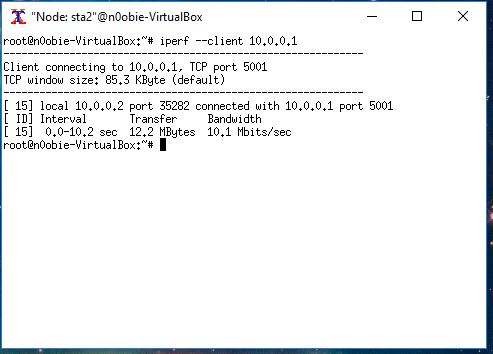
\includegraphics[width=0.7\linewidth]{./img/anexos/4.JPG}
    \caption{Resultados en el cliente.}
  \label{fig:yo}
\end{figure}
\newpage
\chapter{Traza ejecución Mininet-Wifi}
\begin{figure}[!htb]
  \centering
    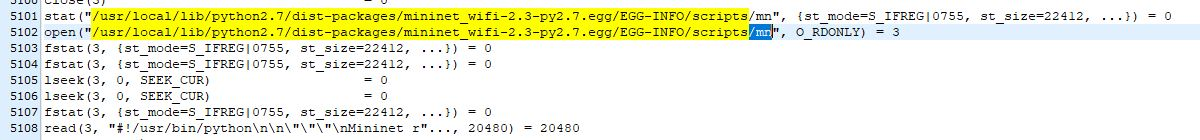
\includegraphics[width=\linewidth]{./img/util/fin.JPG}
    \caption{Llamada al script de Mininet-Wifi (Entrypoint).}
  \label{fig:yo}
\end{figure}
